\documentclass[15pt]{sprawozdanie}
\usepackage{soul}

% \class{Praca dyplomowa inżynierska}
% \title{Opracowanie wirtualnego środowiska do symulacji dynamiki lotu bezzałogowych statków powietrznych}
\class{Projekt zespołowy -- specyfikacja}
\title{Wirtualne środowisko do symulacji dynamiki lotu bezzałogowych statków powietrznych}
\author{\textbf{inż. Wojciech Gajda} 304494\\\vspace{20pt}\textbf{Igor Faliszewski} 313223}
\instructor{dr inż. Paweł Kotowski}
\deadline{\today}

\graphicspath{{images/}}

\usepackage{amssymb}
\usepackage{amsmath}
\usepackage{polski}
\usepackage[utf8]{inputenc}
\usepackage{hyperref}
\usepackage{blindtext}
\usepackage{multicol}
\usepackage{multirow}
\usepackage{wrapfig}
\usepackage{float}
\usepackage{enumitem}
\usepackage{xfrac}
\usepackage{caption}
\usepackage{subcaption}
\usepackage{booktabs}
\usepackage{wasysym}
\usepackage{xcolor}
\usepackage{listings}
\usepackage{pdfpages}
\usepackage{fontspec}
\usepackage{comment}
\usepackage{tocloft}

\setmainfont{Verdana}

\addtolength{\cftsubsecnumwidth}{10pt}
	
\usepackage{color, colortbl}
\definecolor{Gray}{gray}{0.9}

\definecolor{mGreen}{rgb}{0,0.6,0}
\definecolor{mGray}{rgb}{0.5,0.5,0.5}
\definecolor{mPurple}{rgb}{0.58,0,0.82}
\definecolor{backgroundColour}{rgb}{0.95,0.95,0.92}

\lstdefinestyle{CStyle}{
    backgroundcolor=\color{backgroundColour},   
    commentstyle=\color{mGreen},
    keywordstyle=\color{magenta},
    numberstyle=\tiny\color{mGray},
    stringstyle=\color{mPurple},
    basicstyle=\footnotesize,
    breakatwhitespace=false,         
    breaklines=true,                 
    captionpos=b,                    
    keepspaces=true,                 
    numbers=left,                    
    numbersep=5pt,                  
    showspaces=false,                
    showstringspaces=false,
    showtabs=false,                  
    tabsize=2,
    language=C
}

\usepackage[
backend=biber
,style=ieee
,sorting=none
]{biblatex}
\addbibresource{bibliografia.bib}
\DeclareNameAlias{author}{last-first}

\DeclareCiteCommand{\supercite}[\mkbibsuperscript]
  {\iffieldundef{prenote}
     {}
     {\BibliographyWarning{Ignoring prenote argument}}%
   \iffieldundef{postnote}
     {}
     {\BibliographyWarning{Ignoring postnote argument}}}
  {\usebibmacro{citeindex}%
   \bibopenbracket\usebibmacro{cite}\bibclosebracket}
  {\supercitedelim}
  {}
  
  \DeclareLabelalphaTemplate{
  \labelelement{
    \field[final]{shorthand}
    \field{label}
    \field[strwidth=3,strside=left,ifnames=1]{labelname}
    \field[strwidth=1,strside=left,final]{labelname}
    \field{labeltitle}
  }
  \labelelement{
    \field[strwidth=2,strside=right]{year}
  }
}

%\let\cite=\supercite

\renewcommand*{\figurename}{Rys.}

\usepackage{titlesec}
\titlelabel{\thetitle.\quad}

\usepackage{tikz}


\usetikzlibrary{matrix, ,backgrounds}
\usepackage{array}

\makeatletter
\tikzset{SWOT/.style={matrix of nodes,inner sep=0pt,row sep=0pt,column sep=0pt,
cells={nodes={anchor=center,inner sep=2pt}},
column 1/.style={nodes={rotate=90,minimum height=8mm}},
ampersand replacement=\&,
execute at end matrix={\begin{scope}[on background layer]
 \fill[black!10] (\tikz@fig@name.west|-\tikz@fig@name-2-2.north) rectangle 
  (\tikz@fig@name-\the\pgfmatrixcurrentrow-2.south west);
\end{scope}
\draw (\tikz@fig@name.west|-\tikz@fig@name-2-2.north) rectangle 
(\tikz@fig@name-\the\pgfmatrixcurrentrow-\the\pgfmatrixcurrentcolumn.south east)
 (\tikz@fig@name-1-2.north west) rectangle 
(\tikz@fig@name-\the\pgfmatrixcurrentrow-\the\pgfmatrixcurrentcolumn.south east)
(\tikz@fig@name-2-2.center|-\tikz@fig@name.north) --
 (\tikz@fig@name-2-2.center|-\tikz@fig@name.south)
foreach \XX in {2,...,\the\numexpr\pgfmatrixcurrentrow-1}
{(\tikz@fig@name-\XX-2.south-|\tikz@fig@name.west) --
(\tikz@fig@name-\XX-2.south-|\tikz@fig@name.east) };
}}}
\makeatother

\usepackage{tocloft}
\renewcommand\cftfigfont{\small}

\setlength{\parindent}{0pt}

\begin{document}
\maketitle
%
\includepdf[pages=-]{first_page.pdf}


\section*{Streszczenie}
Niniejsza specyfikacja stanowi opis systemu przeznaczonego do symulacji dynamiki lotu bezzałogowych statków powietrznych. System pozwala na prowadzenie symulacji lotu w czasie rzeczywistem, który dodatkowo jest prezentowany jest w postaci trójwymiarowej wizualizacji. W trakcie wykonywania lotu logowane są dane i mogą zostać wykorzystane do analizy lotu. Opracowany został uniwersalny model dynamiki pozwalający na swobodną konfigurację parametrów statku. Obejmuje on modyfikację właściwości mechanicznych, aerodynamicznych oraz konfigurację zespołów napędowych i~wpływu czynników zewnętrznych. Symulacja dynamiki rozszerzona została o system sterowania. System został zaprojektowany w sposobu ułatwiający zmianę parametrów statków i symulacji, tworzenie nowych konfiguracji statków oraz tworzenie i strojenie systemów sterowania. Przykładowych modelami, które mogą zostać zasymulowane są: stałopłatowiec, wielowirnikowiec i rakiety. 

\section*{Słowa kluczowe}

symulacja, grafika komputerowa 3D, bezzałogowy statek powietrzny, model dynamiki ruchu

%\newpage

%\section*{Abstract}

%\section*{Keywords}

\newpage
\tableofcontents

\newpage

\section{Historia zmian}

\renewcommand{\arraystretch}{1.5}
\begin{table}[!h]
\centering
\begin{tabular}{|m{0.12\textwidth}|m{0.12\textwidth}|m{0.20\textwidth}|m{0.45\textwidth}|} 
\hline
\rowcolor{Gray}
Nr rewizji & Data & Autor & Opis \\
 \hline
  0.0 & 10.08.23 & Wojciech Gajda & Utworzenie dokumentu, podstawowa struktura \\ 
\hline
  0.1 & 11.10.23 & Wojciech Gajda & Dostosowanie dokumentu do wymogów edytorskich, dodanie streszczenia \\ 
\hline
  0.2 & 15.10.23 & Wojciech Gajda \newline Igor Faliszewski & Dodanie  słownika, specyfikacji, analizy SWOT i bibliografii \\ 
\hline
  1.0 & 16.10.23 & Wojciech Gajda \newline Igor Faliszewski & Wydanie zgłoszone do L1 \\
\hline
  1.1 & 16.10.23 & Wojciech Gajda \newline Igor Faliszewski & Wprowadzenie poprawek po L1 \\
\hline
  1.2 & 5.11.23 & Wojciech Gajda \newline Igor Faliszewski & Wydanie zgłoszone do L2 \\
\hline
  1.3 & 5.12.23 & Wojciech Gajda \newline Igor Faliszewski & Wydanie zgłoszone do L3/L4 \\
\hline
\end{tabular}
\caption{Historia zmian}
\label{changelog}
\end{table}

\newpage

\section{Słownik pojęć}

\textbf{Statek powietrzny} -- urządzenie zdolne do unoszenia się (lotu) w atmosferze. Statek powietrzny jest zdolny w sposób aktywny wpływać na kierunek i prędkość lotu. W przeciwieństwie do formalnej definicji termin obejmuje również konstrukcję niewykorzystujące oddziaływania powietrza w locie (rakiety).\\

\textbf{Bezzałogowy statek powietrzny, BSP} -- statek powietrzny, który nie wymaga do lotu załogi obecnej na pokładzie oraz nie ma możliwości zabierania pasażerów, pilotowany zdalnie lub wykonujący lot autonomicznie.\\ 

\textbf{Pocisk} -- obiekt wystrzelony lub upuszczony ze statku powietrznego, nieposiadający własnego napędu. Porusza się na wskutek oddziaływania pola grawitacji i wpływu powietrza. Nie posiada wyróżnionej orientacji.\\

\textbf{Ładunek} -- pocisk, na ogół upuszczany, który pozostaje związany z statkiem powietrzanym na sprężysto-tłumiącej linie. \\

\textbf{Stan obiektu} -- Opis położenia, orientacji i prędkości obiektu (pocisku lub statku powietrznego). Stan może zostać rozszerzony o dodatkowe informacje, takie jak: prędkości obrotowe poszczególnych silników, położenie powierzchni sterowych itd. \\

\textbf{Silnik fizyczny, silnik dynamiki} -- program komputerowy, którego zadaniem jest obliczenie położenia, orientacji i prędkości (kinematyki) statków powietrznych w zależności od sił działających na obiekt (dynamiki). \\

\textbf{Regulator} -- układ odpowiedzialny za generowanie rozkazów sterujących w oparciu o aktualny i zadany stan obiektu.\\

\textbf{Silnik graficzny} -- program komputerowy, którego zadaniem jest wizualizacja stanu obiektów i otoczenia.\\

\textbf{Agregator} --  program komputerowy, którego zadaniem jest zarządzaniem stanem aplikacji, obsługa przyłączających się aplikacji klienckich i zarządzanie procesami.\\

\textbf{Zasoby wizualizacji, assety} -- Modele i grafiki niezbędne do pracy aplikacji klienckiej.\\


\newpage

\section{Wstęp}

\subsection{O projekcie}

Symulacje komputerowe dynamiki ruchu stanowią użyteczne narzędzie w pracach inżynierskich. Pozwalają na analizę poprawności działania układu mechanicznego przed jego wyprodukowaniem. W szczególności w zagadnieniu jakim jest projektowanie bezzałogowych statków powietrznych, zastosowanie symulacji pozwala zminimalizować koszty wytworzenia poprawnie działającego systemu.

\subsection{Przegląd istniejących rozwiązań}

Historia symulatorów lotu sięga lat 30. XX wieku. Pierwotnie zastosowanie symulatorów sprowadzało się do szkolenia pilotów cywilnych i wojskowych. W znanej obecnie formie kompletne symulatory lotu stanowią rozbudowane systemy integrujące wysokiej klasy oprogramowanie z peryferiami mającymi wierne odwzorowanie kokpitu kierowanej maszyny. Symulatory wykorzystywane do treningu pilotów podlegają rygorystycznym regulacją prawnym i na ogół ich zadaniem jest odwzorowanie jednej konkretnej maszyny. Równolegle uproszczone wersje symulatorów zaczęły zyskiwać popularność w zastosowaniu cywilnym, jako element rozrywki. W szczególności gry komputerowe związane z lotem bardzo często poświęcały zgodność z rzeczywistością na rzecz lepszych odczuć użytkownika.\\

Na rynku dostępnych jest wiele środowisk symulacyjnych o różnym stopniu szczegółowości. Pełne systemy lotu stanowią produkt komercyjny projektowany na indywidualne zamówienie. Do najpopularniejszych dostępnych systemów sprzedawanych jako zamknięte oprogramowanie należą m. in.:

\begin{itemize}
\item Microsoft Flight Simulator -  seria komputerowych symulatorów lotu pozwalająca na symulację pilotowania różnych statków powietrznych. Założeniem jest wierne odtworzenie zachowania statków powietrznych, warunków pogodowych, jak również samych maszyn,
\item VBS (Arma) - środowisko symulacyjne do wizualizacji pola walki,
\item Warthunder - darmowa gra komputerowa wprowadzająca znaczną ilość historycznych i współczesnych modeli samolotów, których parametry zostały oparte na dostępnych i odtajnionych danych,
\item RealFlight - modelarski symulator lotu.
\end{itemize}

Istnieją również rozwiązania typu open-source, realizujące jedynie poszczególne zadania:

\begin{itemize}
\item JSBsim - rozbudowany silnik dynamiki lotu działający w czasie rzeczywistym,
\item Ardupilot, INAV, Betaflight - kompletne systemy sterowania dla modeli zdalnie sterowanych.
\end{itemize}


\section{Specyfikacja}


\subsection{Cel projektu}

Celem niniejszej projektu jest opracowanie wirtualnego środowiska do symulacji dynamiki lotu bezzałogowych statków powietrznych. System implementuje rozbudowany model dynamiki statków powietrznych wyposażonych w silniki rotorowe, silniki odrzutowe, powierzchnie nośne i powierzchnie sterowe. Pozwala na przeprowadzenie lotu symulowanym obiektem, którego parametry określane są przez konfigurację podaną przez użytkownika. Oprócz lotu system udostępnia dodatkowe funkcjonalności, takie jak możliwość strzału, upuszczenia ładunku, lotu z ładunkiem, rozpoznawania kolizji z otoczeniem.\\

Oprogromowanie ma stanowić zaawansowane narzędzie inżynierskie. Docelowym odbiorcą mają być zespoły R\&D opracowujące nowe konstrukcje latające lub prowadzące prace nad nowatorskimi systemami sterowania. System umożliwia zamodelowanie rzeczywistego modelu latającego i symulację jego lotu przed rzeczywistymi lotami próbnymi, co w rezultacie pozwoli na zminimalizowanie kosztów prototypowania. System rejestruje wiele parameterów lotu umożliwiając późniejszą analizę. Potencjalnymi odbiorcami systemu są uczelnie i instytuty naukowe, a także przedsiembiorstwa prowadzące prace badawczo-rozwojowe. Ze wzgledu na różnorodność zagadnień badanych przez wspomniane zespoły, trudno przygotować oprogramowanie uniwersalne. Z tego powodu system zostanie udostępniony na otwartej licencji MIT, aby umożliwić zespołom dostosowanie go do własnych potrzeb. Dla uławienie dalszego rozwoju projektu duży nacisk położony zostanie na przejrzystą implementację i realizację wzorców możliwych do ponownego użycia.\\

Otwarta licencja umożliwa również wykorzystanie systemu do celów rekreacyjnych i hobbistycznych. Szczególnym przypadkiem są modelarze, posiadający nierzadko znaczną wiedzę domenową i budujący swoje modele ze znaczną dbałością o szczegóły. Projektowany system może stanowić dla nich zamiennik profesjalnego oprogramowania, które ze względu na koszty licencji pozostawało dla nich niedostępne. Specyfika oprogramowania pozwala na użytkowanie go również w roli gry komputerowej. Oprócz wartości rozrywkowej, korzystanie z symulatora pozwala rozwijąc umiejętności pilotarzu, co przenosi się na rzeczywiste modele. Planowane jest wprowadzenie kilku funkcjonalności, których rolą jest jedynie poleszenie odczuć użytkonika aplikacji i zwiększenie przyjemności z korzystania z systemu.\\

\newpage
\subsection{Wymagania funkcjonalne}

Wyróżniono trzech aktorów korzystających z systemu: Użytkownika, Analityka i Developera. Użytkownik to osoba o najmniejszej wiedzy domenowej. Korzysta z systemu odpowiednio skonfigurowanego i przygotowanego. Rolą Użytkownika jest wykonywanie lotów i realizacja określonej misji. Można porównać go do gracza. Użytkownik korzysta z systemu, aby nauczyć się pilotować określony BSP lub aby trenować zaawansowane manewny, np. atak na poruszający się cel lub precyzyjne upuszczenie ładunku. Analityk to osoba posiadająca rozbudowaną wiedzę teoretyczną z zakresu lotnictwa. Odpowiedzialny jest za identyfikacje i wprowadzenie parameterów modelu BSP i przygotowanie konfiguracji do lotu. Po odbytym locie może zwalidować poszczególne aspekty lotu poprzez analizę zarejestrowanych logów. Developer to osoba posiadająca podstawową wiedzę domenową i rozumie kod źródłowy systemu. Rolą developera jest dostosowanie systemu na potrzeby swojego przedsiębiorstwa. Zakłada się, że głowną modyfikacją jest implementacja własnych algorytmów sterowania. Developer ma dostęp do całego kodu źródłowego, przez co jego możliwości są nieograniczone.\\

\textbf{Użytkownik:}
\begin{itemize}[noitemsep,nolistsep]
	\item może uruchomić symulację lotu,
	\item może wybrać jedną z dostępnych konfiguracji BSP,
	\item może dołączyć do symulacji wraz z innymi użytkownikami,
	\item może dodać konfigurację własnego kontrolera
	\item może w trakcie lotu wystrzelić pocisk,
	\item może w trakcie lotu upuścić ładunek i przenosić go na elastycznej linie,
	\item może zderzyć się z ścianmi mapy, innym BSP lub pociskiem,
	\item może połączyć się zdalnie z wykorzystaniem protokołu TCP/IP,
	\item może odczytać stan swojego BSP z GUI,
	\item może zmienić widok z kamery,
	\item może uruchomić radio w grze.
\end{itemize}
\ \\

\textbf{Analityk:}
\begin{itemize}[noitemsep,nolistsep]
	\item może przygotować nową konfigurację drona,
	\item może analizować logi z wykonanych lotów,
	\item może zaplanować otoczenie symulacji, wybrać mapę i ustalić warunki atmosferyczne.
\end{itemize}
\ \\

\textbf{Developer:}
\begin{itemize}[noitemsep,nolistsep]
	\item może dodać i zarządzać istniejącymi algorytmami sterowania,
	\item implementować nowe funkcjonaloności systemu.
\end{itemize}
\ \\


\newpage
\subsection{Wymaganie niefunkcjonalne}

W tabeli (\ref{non_func}) przedstawiono wymagania niefunkcjonalne, które musi spełniać oprogramowanie.

\renewcommand{\arraystretch}{1.5}
\begin{table}[!h]
	\centering
	\begin{tabular}{|m{0.03\textwidth}|m{0.21\textwidth}|m{0.025\textwidth}|m{0.68\textwidth}|} 
		\hline
		\rowcolor{Gray}		\multicolumn{2}{|c|}{Wymagania} & No. & Opis \\
		\hline
		\centering \multirow{9}{*}{\rotatebox[origin=c]{90}{Usability}}
		&\multirow{1}{*}{Używalność} 
		& 1 & Użytkownik jest w stanie dopasować rozmiar okna wizualizacji i interfejsu do swoich potrzeb i ograniczeń sprzętu. \\
		\cline{3-4}
		& & 2 & Serwer da się uruchomić natywnie na Unixie lub w wirtualnym kontenerze Docker, a wizualizacja działa na wirtualnej maszynie Javy. \\
		\cline{3-4}
		& & 3 & Komunikacja między serwerem, a wizualizacją powinna pozwalać na responsywne sterowanie BSP. \\
		\cline{2-4}
		& \multirow{1}{*}{Ergonomia} 
		& 4 & Interfejs użytkownika powinien być przejrzysty i korzystać ze standardowych liczników wykorzystywanych w~lotnictwie.  \\
		\cline{3-4}
		& & 5 & Konfiguracja kontrolera powinna odbyć się bez znajomości użytkownika z interpretacją wejścia przez system.  \\
		\hline
		\centering \multirow{3.5}{*}{\rotatebox[origin=c]{90}{Reliability}}
		& \multirow{1}{*}{Dokładność} 
		& 6 & Dokładność symulacji powinna zależeć wyłącznie od błędów obliczeń i dokładności wprowadzonych parametrów. \\
		\cline{2-4}
		& \multirow{1}{*}{Sprawdzalność} 
		& 7 & Zgodność symulacji z rzeczywistością da się sprawdzić poprzez analizę logów oraz przez subiektywną opinię analityka. \\
		\hline
		\centering \multirow{1}{*}{\rotatebox[origin=c]{90}{Perf.}}
		& \multirow{1}{*}{Przepustowość} 
		& 8 & Wydajność serwera powinna skalować się względem liczby aktualnie symulowanych BSP. \\
		\hline
		\centering \multirow{7}{*}{\rotatebox[origin=c]{90}{Supportability}}
		& \multirow{1}{*}{Konserwacja} 
		& 9 &Systemy sterowania, elementy interfejsu i moduły konfigurowalne powinny być tak zaprojektowanie aby dodawanie nowych oraz modyfikacja istniejących była prosta i szybka.  \\
		\cline{3-4}
		& & 10 & System powinien być podzielony na moduły, które można niezależnie modyfikować. \\
		\cline{2-4}
		& \multirow{1}{*}{Audytowalność} 
		& 11 & W czasie lotu serwer powinien zapisywać logi z symulacji. \\
		\cline{2-4}
		& \multirow{1}{*}{Instalowalność} 
		& 12 & Proces instalacji serwera powinien być dobrze opisany i~prosty. Niewymagany w przypadku wizualizacji. \\
		\cline{2-4}
		& \multirow{1}{*}{Konfigurowalność} 
		& 13 & Oprogramowanie powinno umożliwiać konfigurację serwera, wizualizacji, modeli, kontrolerów, parametrów BSP. \\
		\hline
	\end{tabular}
	\caption{Wymaganie niefunkcjonalne - FURPS}
	\label{non_func}
\end{table}

\subsection{Architektura}

System został podzielony na moduły. Poszczególne moduły odpowiadają obiektom z domeny projektu i realizują następujące zadania:\\

\textbf{UAV\_physic\_engine} -- moduł odpowiedzialny symulację dynamiki statku powietrznego, uwzględniając wszystkie jego własciwości mechaniczne i wpływ otoczenia. Oblicza stan pojedynczego BSP w czasie rzeczywistym. \\

\textbf{UAV\_controller} -- moduł reprezentujący system sterowania statkiem powietrznym. Interpretuje stan statków powietrznych i buduje symulacje otoczenie. Symuluje działanie czujników pomiarowych, systemu filtracji, algorytmów nawigacji pokładowej oraz systemów sterowania i stabilizacji. Bezpośrednio wpływa na zachowanie symulacji dynamiki.\\

\textbf{UAV\_drop\_physic} -- moduł odpowiedzialny za obliczenie dynamiki pocisków. Oblicza stan wszystkich pocisków aktywnych w symulacji.\\

\textbf{UAV\_aggregator} -- moduł agregujący moduły symulacyjne z wizualizacją. Zarządza pracą pozostałych modeli i wprowadza niektóre zagadnienia otoczenia takie jak atmosferę, połączenia miedzy BSP, a ładunkami oraz kolizje.\\

\textbf{UAV\_server} -- definicja wirtualnego kontenera, odpowiedzialna zabudowanie wszystkich modułów składających się na serwer, tj. wszystkie z wyłączeniem wizualizacji. Ze zbudowanych modułów budowany jest obraz kontenera. Umożliwia to uruchomienie serwera na dowolnej maszynie wspierającej daną konteneryzację.\\

\textbf{UAV\_visualization} -- moduł odpowiedzialny za wyświetlenie  interfejsu użytkownika oraz obecnego stanu symulacji. Przekazuje dane wejściowe z kontrolera do systemu. Stanowi interfejs komunikacji użytkownika z systemem. \\

\newpage

\subsection{Opis działania systemu}

W centralnym punkcie aplikacji znajduje się moduł agregatora. Stanowi on główną część serwera, jest aplikacją konsolową i nie posiada interfejsu graficznego. Jest zawsze uruchamiany jako pierwszy. Po rozpoczęciu pracy aggregatora, uruchamiany jest moduł "drop physic" jako podproces, a aggregator nawiązuje z nim połączenie. Oba moduły pozostają w stanie bezczynności do momentu podłączenia się pierwszego użytkownika. Nowy użytkownik dodawany jest przez uruchomienie wizualizacji. Po uruchomieniu wizualizacji, komunikuje się ona z serwerem i prosi o~utworzenie nowego statku powietrznego. W odpowiedzi na to żądanie, aggregator uruchamia jako swoje podprocesy "physic engine" i "controller".Następnie para procesów synchronizuje się ze sobą i rozpoczyna symulację. Każdemu symulowanemu statkowi powietrznemu odpowiada para procesów "physic engine" i "controller". Ponadto, każdy statek jest kontrolowany z poziomu konkretnej wizualizacji.\\

W trakcie pracy systemu, aggregator pełni rolę pośrednika w komunikacji między wizualizacją a procesami silnika fizycznego i regulatora. Przesyła instrukcje sterujące z wizualizacji do odpowiedniej symulacji fizycznej, agreguje stany ze wszystkich aktywnych symulacji i przesyła je z powrotem do wizualizacji. Ponadto, zarządza procesami strzału, upuszczania ładunku i kolizji.\\

Po odłączeniu się wizualizacji od serwera, procesy związane z danym statkiem są zamykane.


\subsection{Opis komponentów}

Kod poszczególnych modułów systemu został w całości opisany z wykorzystaniem narzędzi do dokumentowania kodu: Doxygen, JavaDoc i Rust Doc. Dla poszczególnych modułów wygenerowane zostały opisy klas oraz funkcji i załączone do pracy jako dokumenty PDF lub strony HTML.

\newpage

\subsection{Komunikacja}

Moduły komunikują się między sobą poprzez kolejki ZeroMQ\cite{zmqguide}. ZeroMQ to uniwersalna implementacja różnych wzorów komunikacji niezależna od języka i warstwy transportowej. Istnieją oficjalne biblioteki ZeroMQ przeznaczone do wykorzystania w projektach w językach  C++, Rust, Java, Python i wielu innych. Jako warstwa transportowa wykorzystane mogą być mechanizmy komunikacji wewnątrzprocesowej, międzyprocesowej i protokół TCP/IP oraz dowolne ich kombinację. Wzorami dostępnymi w kolejkach ZeroMQ, które zostaną wykorzystane w projekcie są:

\begin{itemize}
\item PUB--SUB -- jednokierunkowa komunikacja publikujący --  subskrybujący. Jest to połączenie jeden do wielu.  Wielu subskrybujących ma możliwość podłączenia się do jednego publikującego i zasubskrybowania określonych wiadomości (zdefiniowanych przez prefix). Publikujący rozsyła wiadomości do wszystkich podłączonych subskrybentów, którzy subskrybują dany typ wiadomości.

\item PAIR--PAIR -- uniwersalne połączenie jeden do jeden. Tworzy połączenie dwóch socketów, umożliwiające dwukierunkową komunikacje. Stanowi bezpośredni odpowiednich Unixowych pipe'ów lub surowego protokołu TCP.

\item REQ--REP -- model komunikacji klient serwer w której serwer (REP -- replyer) odpowiada na zapytania klienta (REQ -- requester). W modelu wielu klientów może odpytywać serwer, a ich żądania są kolejno obsługiwane i wysyłana jest na nie odpowiedź.
\end{itemize}

Oprócz wyżej przedstawionych istnieje również wiele wariacji modeli komunikacji pozwalające m. in. na rozdzielanie pracy na wiele serwerów (load balance) lub przekierowywanie wiadomości ze zmianą warstwy transportowej lub podsłuchem (proxy).\\

Rysunek (\ref{comm}) prezentuje poszczególne moduły oraz kanały komunikacji. Na niebiesko zaznaczone zostały kolejki TCP/IP, a na czerwono kolejki wykorzystujące mechanizmy IPC. Dla zwiększenia czytelności, kolejki w warstwie miedzy procesowej nie zostały zaznaczone na rysunku.

\newpage
 \begin{figure}[!h]
  \centering
  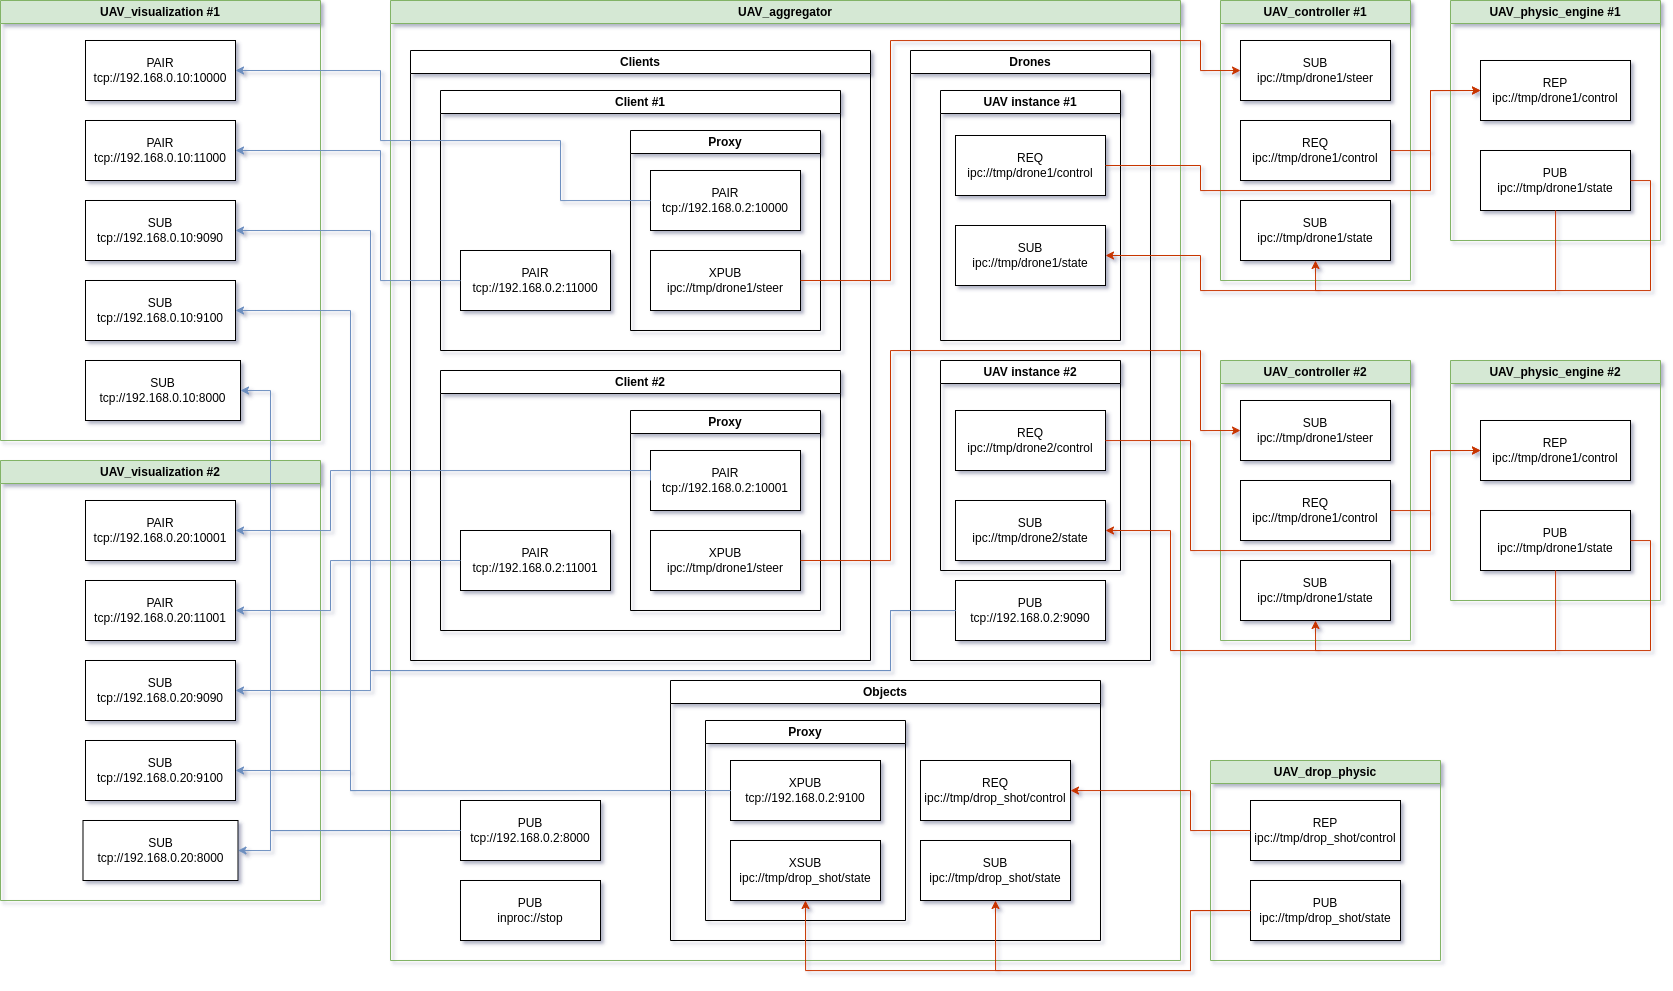
\includegraphics[width=1.2\textwidth, angle=90]{ZMQinMINIUAV.drawio.png}
  \caption{Schemat komunikacji}
  \label{comm}
 \end{figure}

\newpage

\subsection{Graficzny interfejs użytkownika}

Graficzny interfejs użytkownika składa się z interfejsu serwera oraz interfejsu wizualizacji. 

\subsubsection*{Serwer}

Interfejs serwera zawiera komunikaty dotyczące pracy agregatora oraz otrzymywane od poszczególnych modułów, które są wyświetlane w oknie konsoli. Komunikaty są dodatkowo oznaczone kolorami różniącymi dla poszczególnych modułów, jak pokazano na rysunkach (\ref{gui_server1}), (\ref{gui_server2}) i (\ref{gui_server3}).

\subsubsection*{Wizualizacja}

Interfejs graficzny wizualizacji składa się z okna konfiguracji przypisań kontrolera pokazanego na rysunku (\ref{gui_bindings1}), ekranu ładowania widocznego na rysunku (\ref{gui_loading}) oraz właściwego widoku wizualizacji ukazanego na rysunkach (\ref{gui_game1}), (\ref{gui_game2}), (\ref{gui_game3}) i (\ref{gui_game4}). \\

Graficzny interfejs użytkownika w wizualizacji składa się z widoku jednej z kamer do wyboru oraz kokpitu. Kokpit w lewym dolnym rogu zawiera radar pozwalający na wykrycie BSP w okolicy. W prawym dolnym rogu znajduje się schemat silników BSP, gdzie możemy odczytać ich prędkości obrotowe. W prawym górnym rogu jest pokazany stan wyposażenia kontrolowanego BSP. Ponadto na kokpicie na dole ekranu znajduje się sztuczny horyzont, którego wizualizacja zgodna jest z powszechnie stosowaną konstrukcją. Pozwala on na uzyskanie informacji o pozycji BSP w przestrzeni, jego orientacji i prędkościach. W lewym górnym rogu sztucznego horyzontu znajduje się obecny tryb lotu BSP. Użytkownik może również włączyć tryb mapy, aby zobaczyć swoje położenia w świecie symulacji.

\newpage
\begin{figure}[!h]
	\centering
	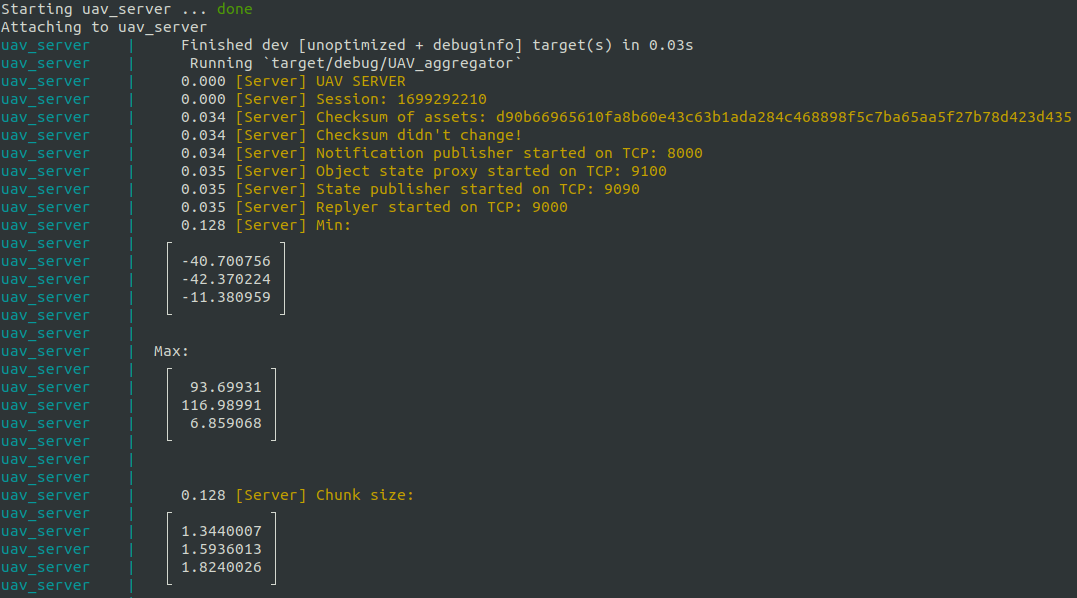
\includegraphics[width=1\textwidth]{gui_server_start.png}
	\caption{Interfejs graficzny serwera w momencie startu.}
	\label{gui_server1}
\end{figure}

\begin{figure}[!h]
	\centering
	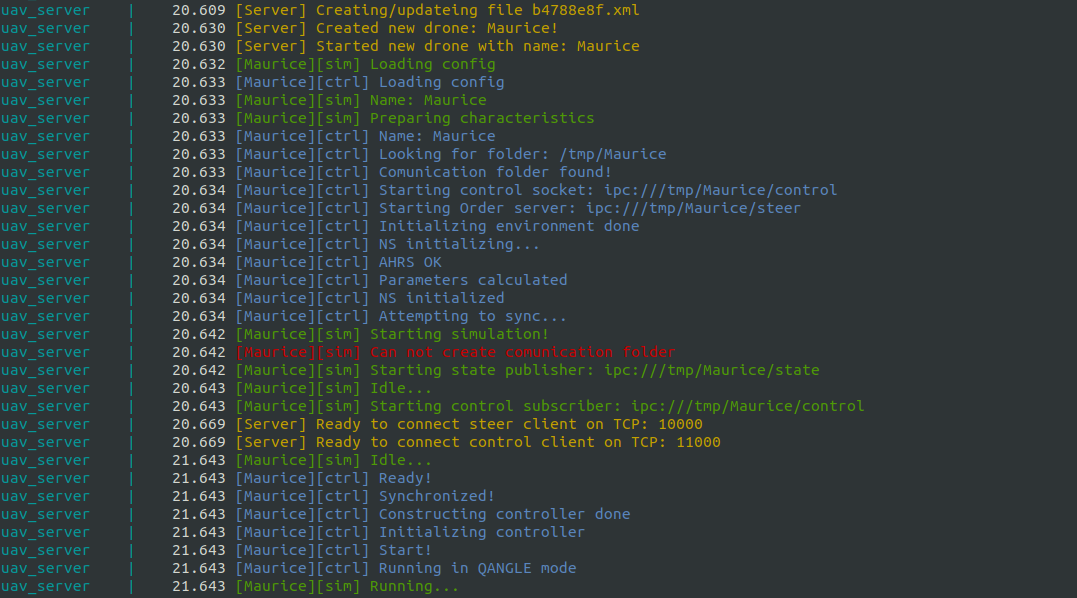
\includegraphics[width=1\textwidth]{gui_server_drone.png}
	\caption{Interfejs graficzny serwera w momencie dołączenia nowego klienta wizualizacji.}
	\label{gui_server2}
\end{figure}

\begin{figure}[!h]
	\centering
	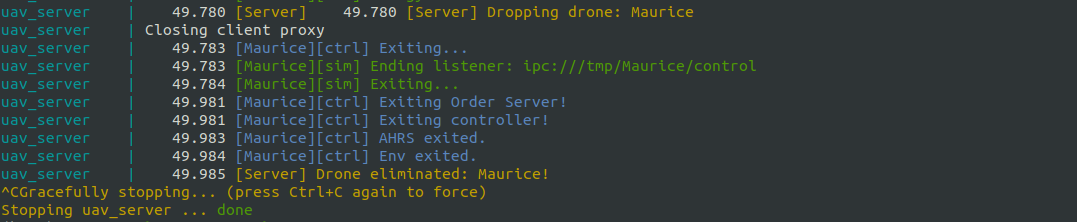
\includegraphics[width=1\textwidth]{gui_server_exit.png}
	\caption{Interfejs graficzny serwera w momencie wyłączenia serwera.}
	\label{gui_server3}
\end{figure}
\begin{figure}[!h]
	\centering
	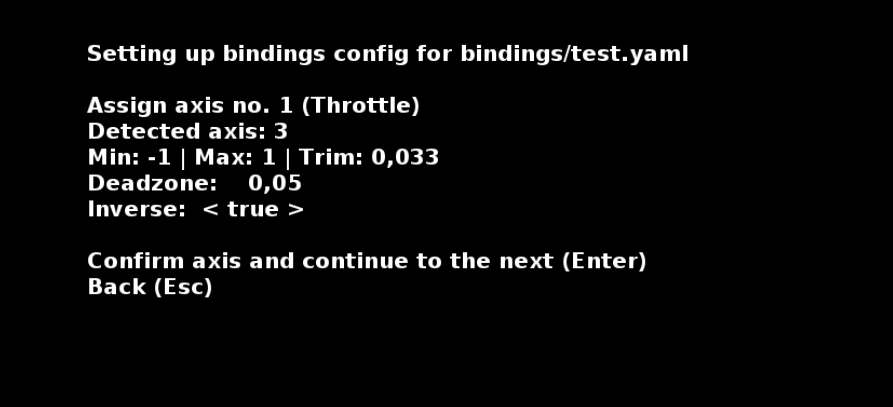
\includegraphics[width=1\textwidth]{bindings1.png}
	\caption{Ekran przypisania osi sterowania.}
	\label{gui_bindings1}
\end{figure}

\begin{figure}[!h]
	\centering
	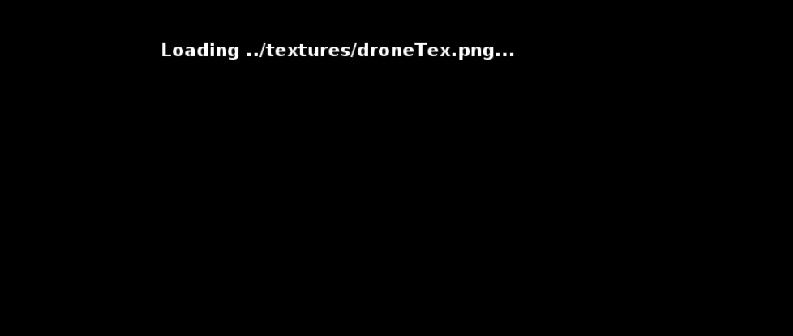
\includegraphics[width=1\textwidth]{loading_screen.png}
	\caption{Ekran ładowania.}
	\label{gui_loading}
\end{figure}

\newpage
\begin{figure}[!h]
	\centering
	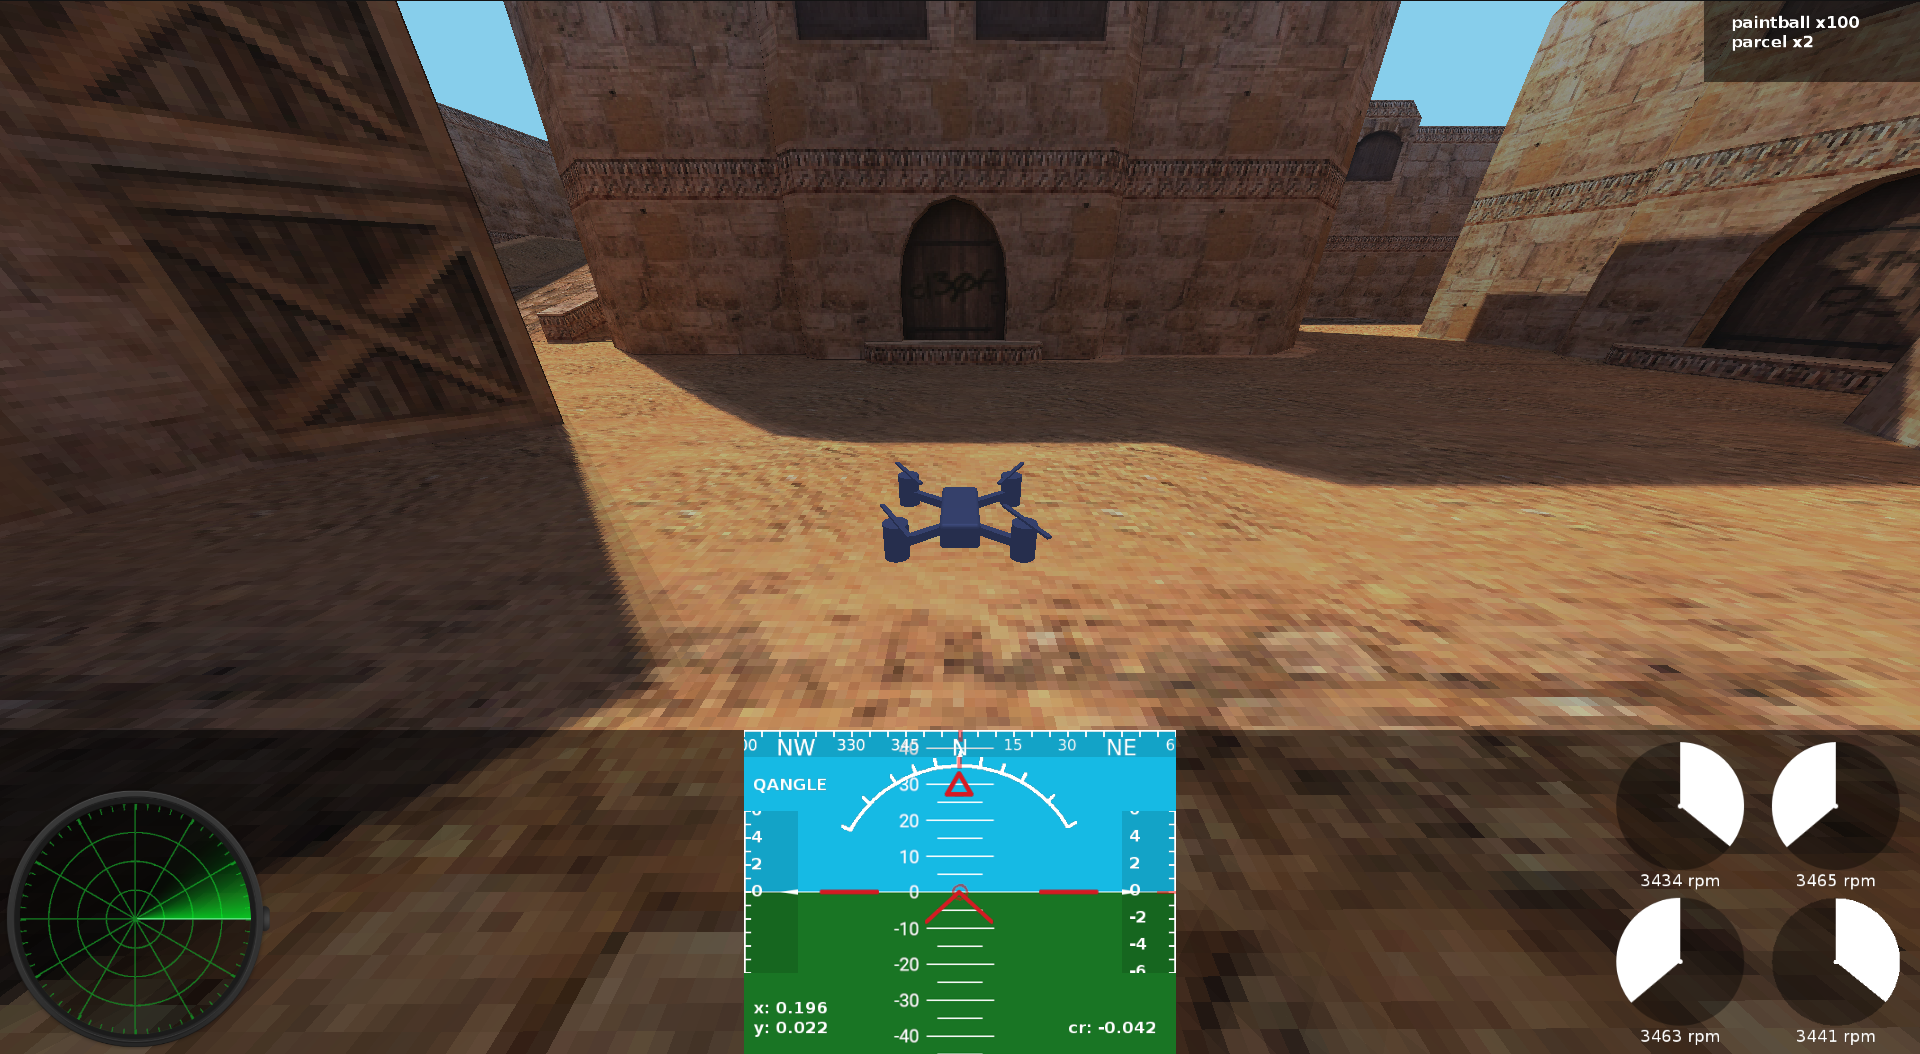
\includegraphics[width=1\textwidth]{game_view.png}
	\caption{Interfejs graficzny wizualizacji w widoku trzecioosobowym.}
	\label{gui_game1}
\end{figure}

\begin{figure}[!h]
	\centering
	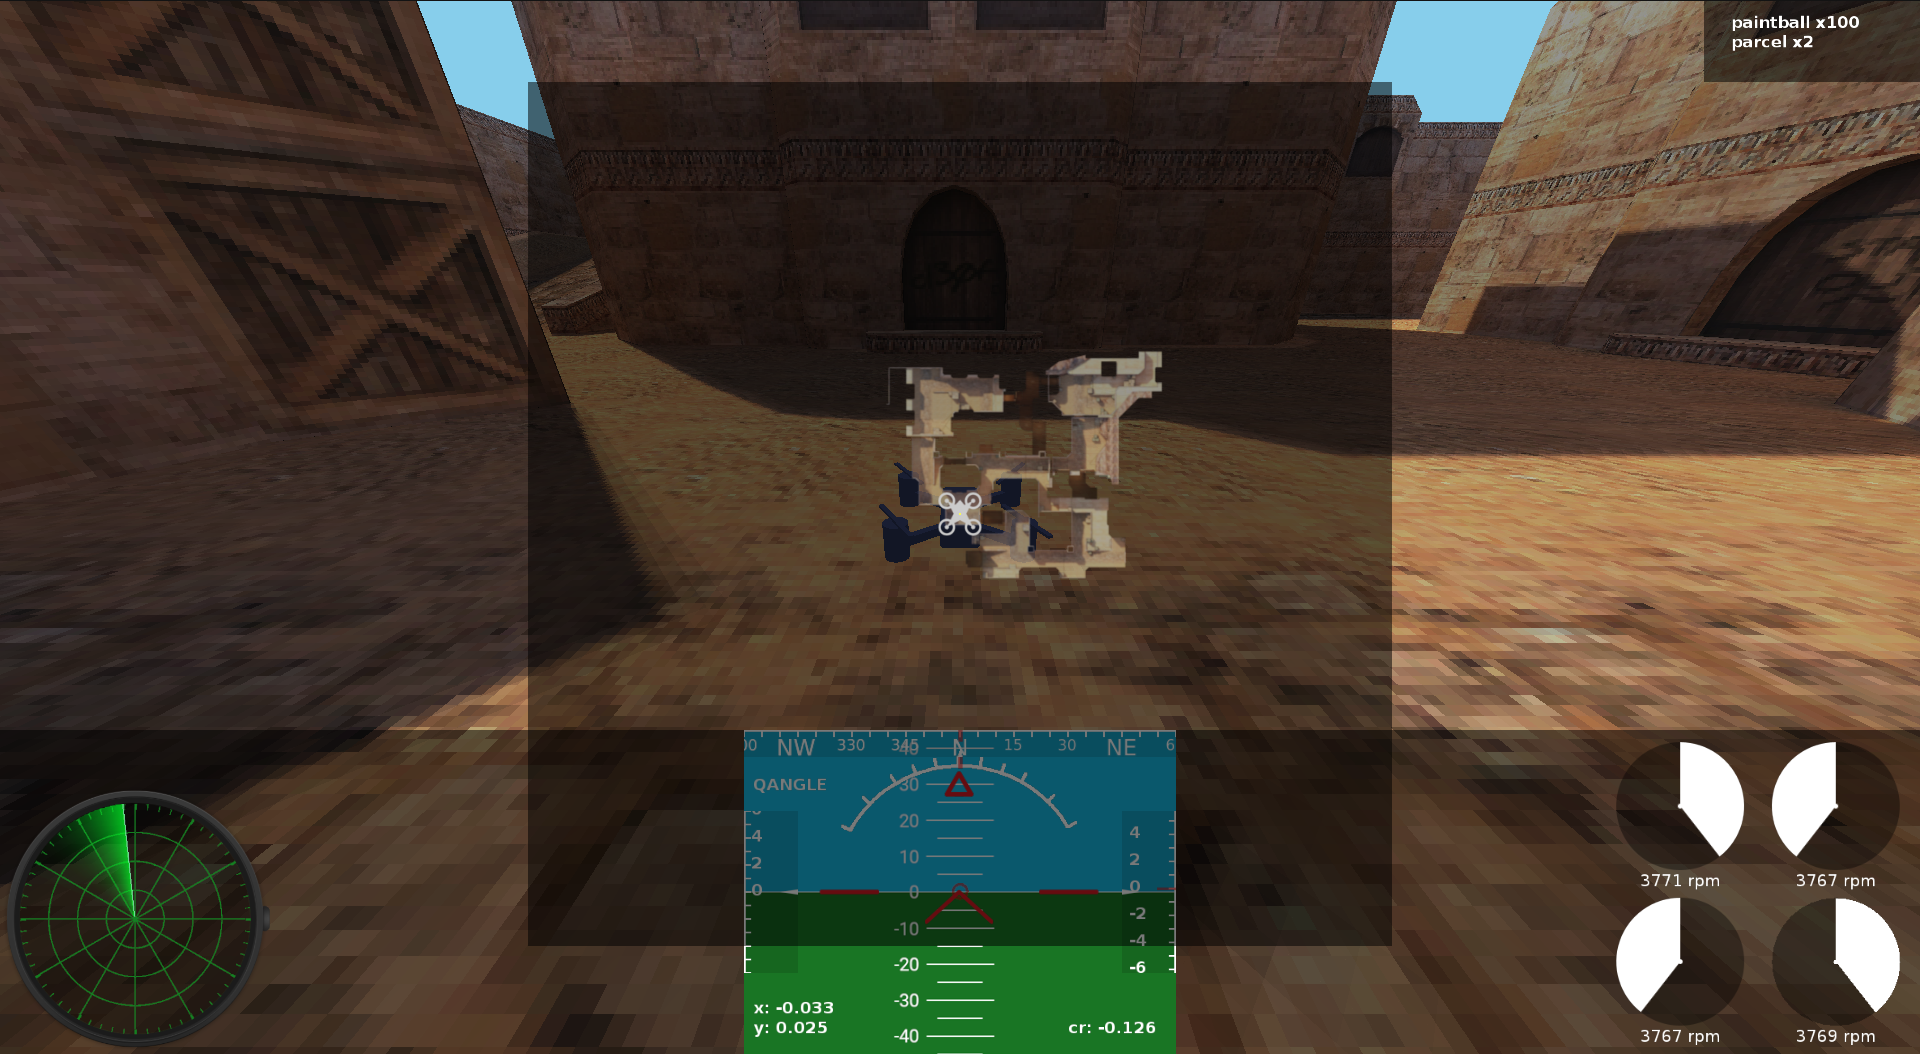
\includegraphics[width=1\textwidth]{game_view_map.png}
	\caption{Interfejs graficzny wizualizacji z włączonym widokiem mapy.}
	\label{gui_game2}
\end{figure}

\newpage
\begin{figure}[!h]
	\centering
	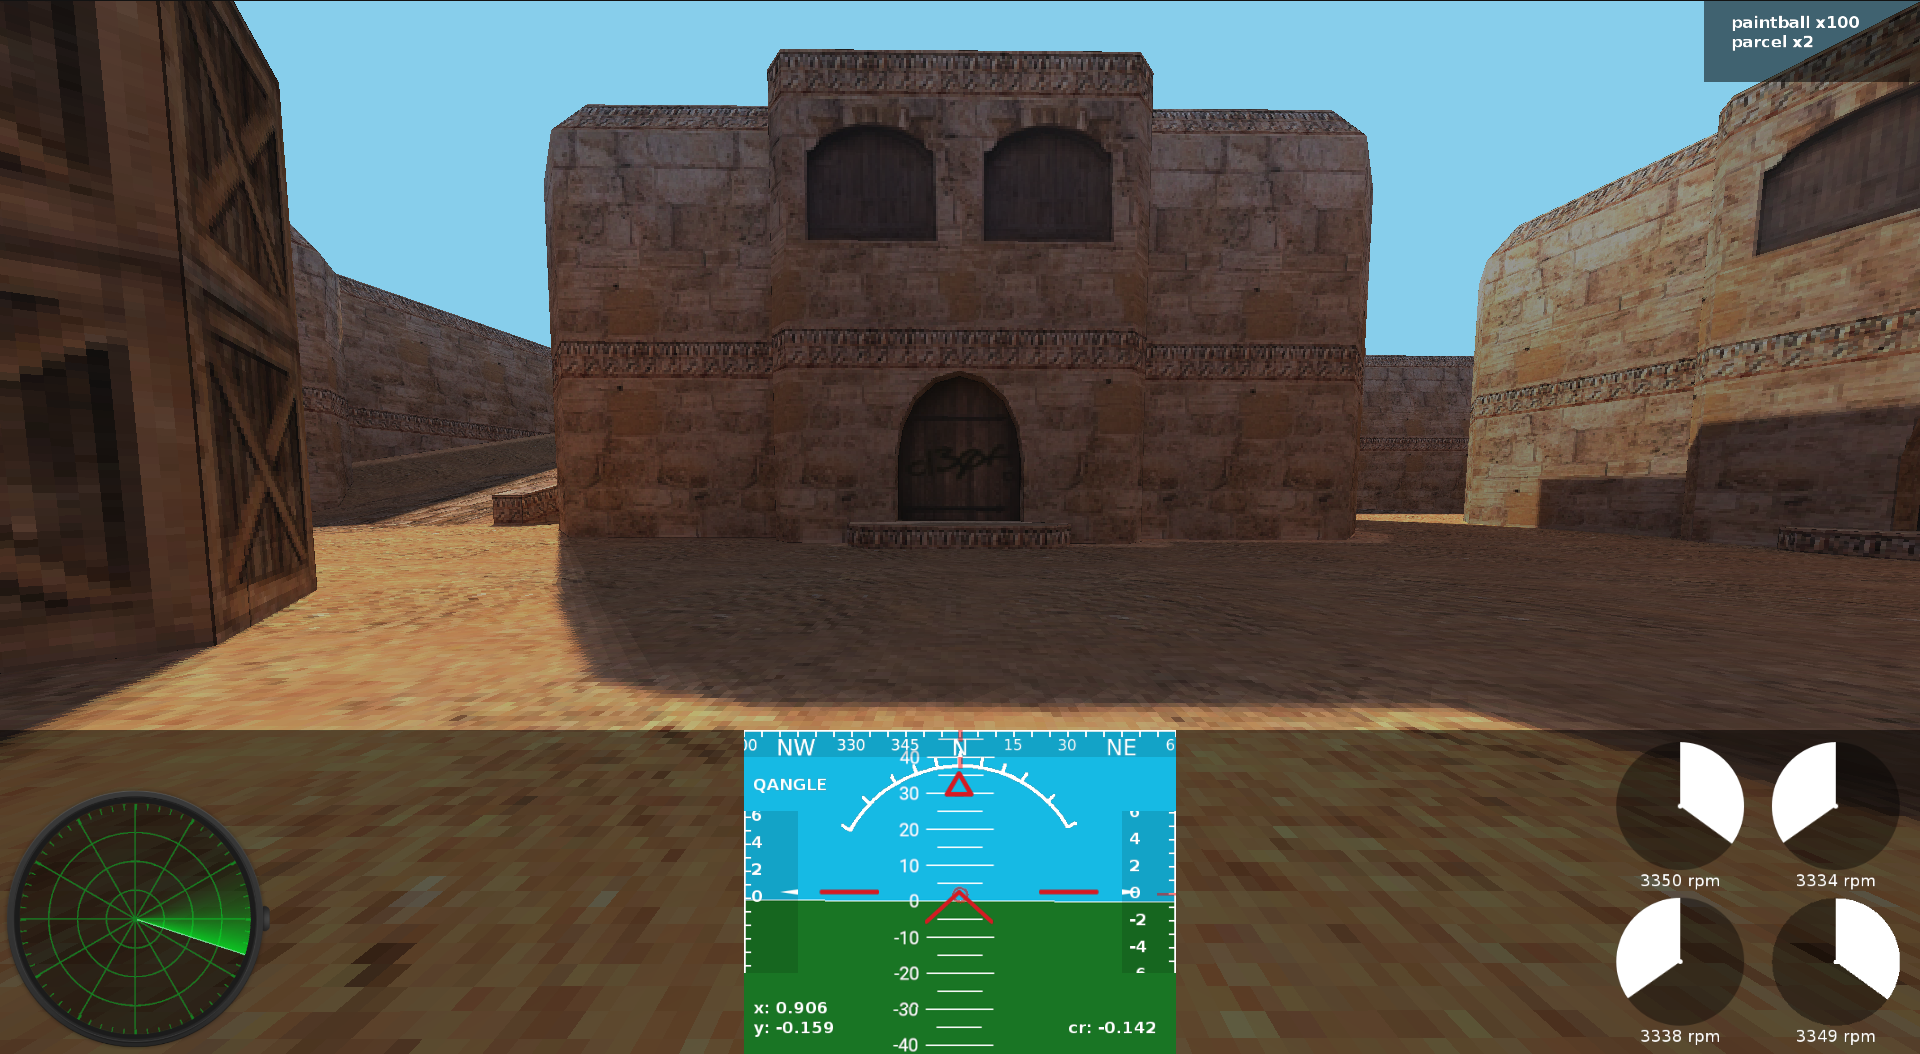
\includegraphics[width=1\textwidth]{game_view_fpp.png}
	\caption{Interfejs graficzny wizualizacji w widoku pierwszoosobowym.}
	\label{gui_game3}
\end{figure}

\begin{figure}[!h]
	\centering
	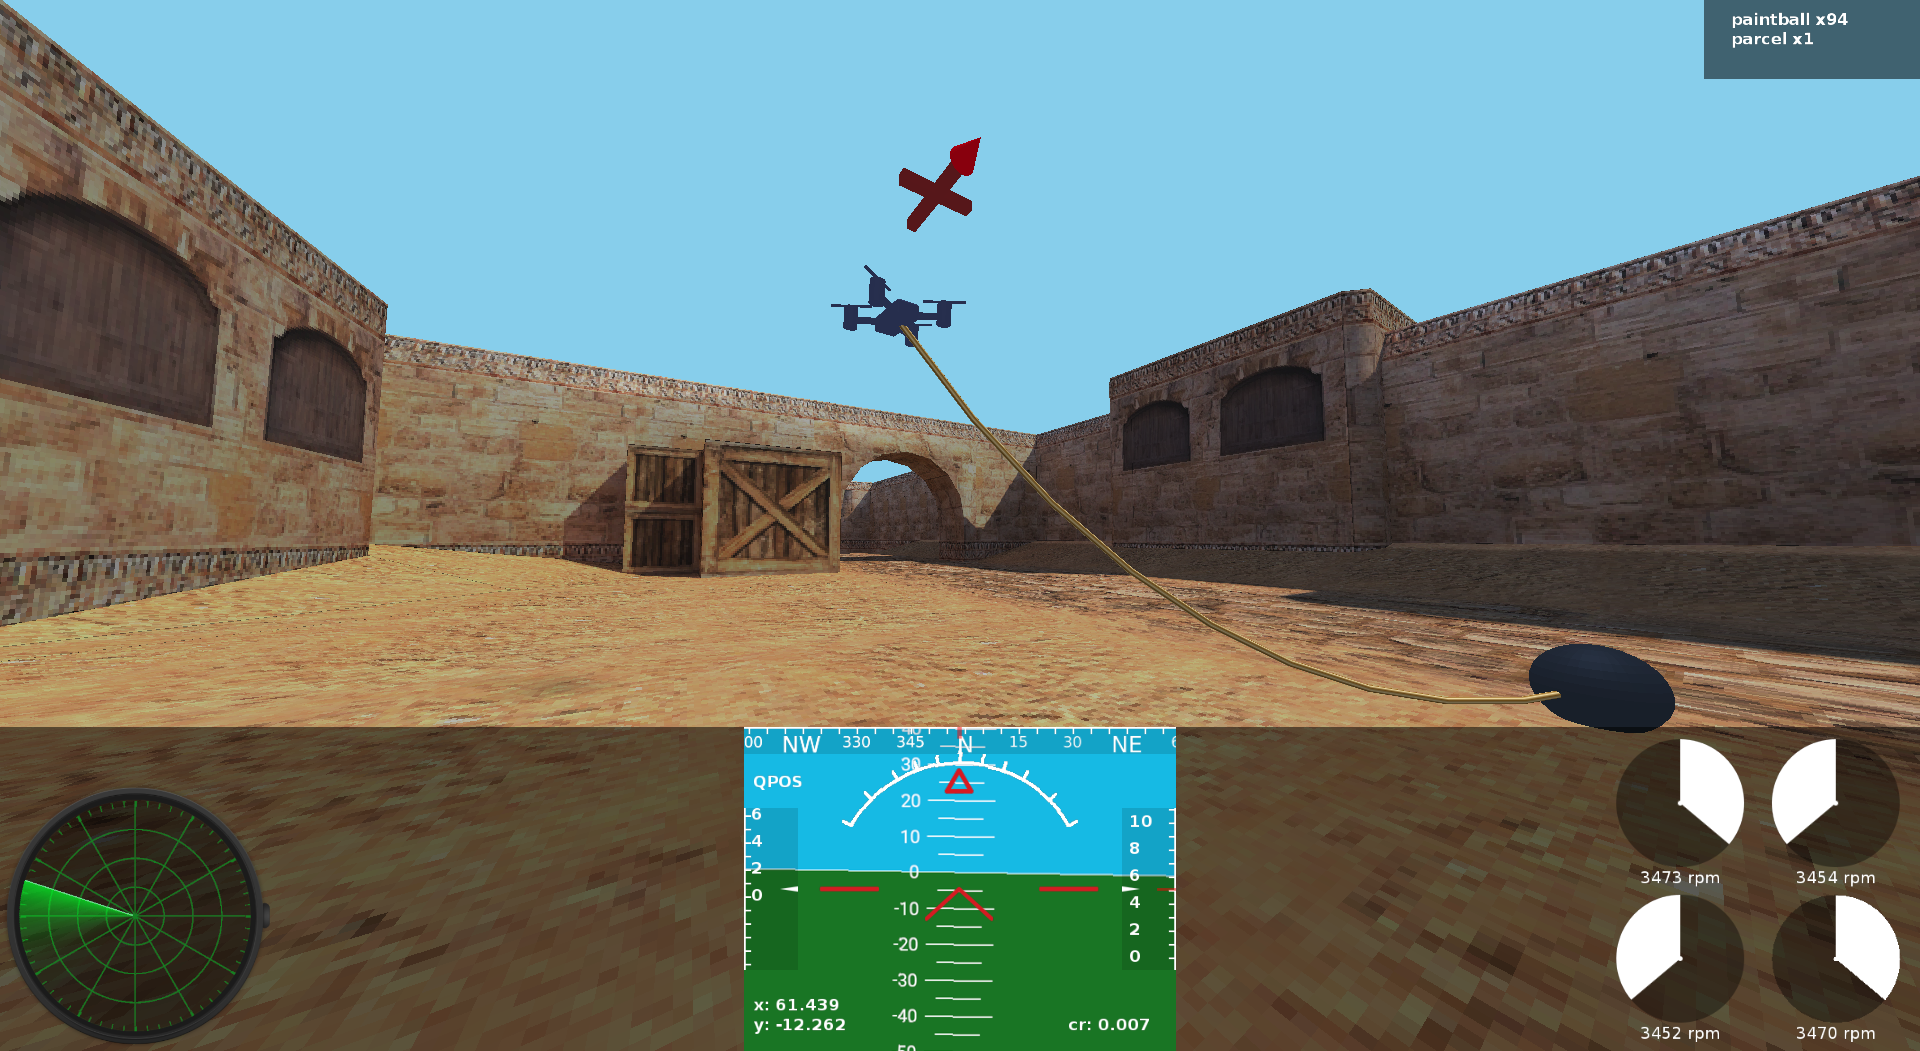
\includegraphics[width=1\textwidth]{game_view_rope.png}
	\caption{Interfejs graficzny wizualizacji w widoku obserwatora i pozycyjnym trybie lotu z opuszczonym ładunkiem na linie.}
	\label{gui_game4}
\end{figure}

\newpage
\subsection{Interfejs zewnętrzny}

Konfiguracja systemu przed uruchomieniem odbywa się poprzez modyfikację plików konfiguracyjnych i zasobów (asset'ów). Pliki konfiguracyjne dotyczą:

\begin{itemize}
\item Parametrów symulowanego statku powietrznego --\\ UAV\_aggregator/configs/template.xml
\item Parametrów agregatora -- UAV\_aggregator/configs/config.yaml
\item Parametrów wizualizacji -- UAV\_visualization/config.yaml
\item Parametrów kontrolera --  UAV\_visualization/bindings/template.yaml
\item Opisu dostępnych trybów lotu --\\ UAV\_aggregator/assets/data/available\_control\_modes.yaml
\end{itemize}

Pliki konfiguracyjne zostały w całości skomentowane przy pomocy komentarzy odpowiednich dla plików XML oraz YAML  i załączone do pracy.\\


Zasoby zawierają modele i grafiki niezbędne do pracy wizualizacji. Wersja zasobów to pierwsze 8 znaków sumy kontrolnej, która jest generowana na podstawie zawartości assetów i przekazywana wizualizacji przez serwer. Pozwala to użytkownikowi pobrać brakujące zasoby w razie, gdy ich jeszcze nie posiada. Pobrana zawartość jest umieszczana w katalogu od nazwie będącej wersją zasobu. Zasób zawiera następujące katalogi:

\begin{itemize}

\item \textbf{Drones} -- folder zawierający modele 3D statków powietrznych. Zawiera foldery odpowiadające poszczególnym BSP. Nazwa folderu jest tożsama z nazwą BSP.
\begin{itemize}
\item \textbf{\textbf{\textit{NazwaModeluBSP}}} -- Katalog zawierający modele wraz z teksturami dla konkretnego modelu BSP w folderach \textbf{model} i \textbf{textures}.
\end{itemize}

\item \textbf{Maps} -- folder zawierający modele 3D map, które mogą zostać wykorzystane w symulacji. Zawiera foldery odpowiadające poszczególnym mapą. Nazwa folderu jest tożsama z nazwą mapy.
\begin{itemize}
	\item \textbf{\textbf{\textit{NazwaMapy}}} -- Katalog modeli danej mapy. Zawiera modele oraz tekstury mapy w folderach \textbf{model} i \textbf{textures}. W folderze \textbf{model} dodatkowo znajduje się obraz mapy z lotu ptaka pod nazwą "minimap.png".
\end{itemize}

\item \textbf{Data} -- folder zawierający wspólne pliki konfiguracyjne. Obecnie zawiera następujące pliki:
\begin{itemize}
	\item "available\_control\_modes.yaml" -- Plik konfiguracyjny zawierający dozwolone tryby kontroli lotu.
\end{itemize}

\item \textbf{Core} -- folder zawierający pozostałe modele 3D i elementy interfejsu. Zawiera następujące podfoldery:
\begin{itemize}
	\item \textbf{GUI} -- Grafiki niezbędne do wyświetlenia elementów interfejsu graficznego użytkownika.
	\item \textbf{projectile} -- Model i tekstury pocisku w katalogach \textbf{model} i \textbf{textures}.
	\item \textbf{xMark} -- Model i tekstury markera 3D w katalogach \textbf{model} i \textbf{textures}.
\end{itemize}

\end{itemize}

W katalogach \textbf{model} zawarty jest model obiektu w postaci pliku z rozszerzeniem GLTF, a więc "model.gltf" wraz z odpowiadającym mu "model.bin" oraz pliku z rozszerzeniem OBJ: "model.obj". Plik GLTF wykorzystywany jest w wizualizacji, a OBJ służy rozpoznawaniu kolizji.\\


W zasobie znajduje się również tekstura domyślna ładowana w przypadku nieznalezienia wymaganej tekstury.\\


\newpage


\subsection{Dobór technologii}

Do realizacji poszczególnych modułów wybrane zostały następujące narzędzia programistyczne i biblioteki zewnętrzne.\\


\textbf{UAV\_physic\_engine, UAV\_controller i UAV\_drop\_physic}\\

Ze względu na duży nakład obliczeniowy -- symulacja w czasie rzeczywistym z krokiem całkowania rzędu 1ms -- wybrany został język C++. Z uwagi na swoją wydajność i elastyczność stanowi on naturalny wybór w wydajnych symulacjach komputerowych. Dodatkowo wykorzystane zostały następujące biblioteki:
\begin{itemize}[noitemsep,nolistsep]
	\item Eigen -- biblioteka zawierająca elementy algebry liniowej: macierze, wektory i~związane z nimi algorytmy. Eigen stawia na wydajność poprzez wykorzystanie rozkadów typu SIMD, przy 		jednoczesnym zachowaniu przejrzystej składni,
	\item ZeroMQ -- binding biblioteki libzmq dla języka C++. Libzmq jest bazową biblioteką implementującą kolejki ZeroMQ w języku C,
	\item RapidXML -- biblioteka do parsowania plików XML,
	\item Cxxopts -- biblitoteka do interpretowania argumentów wejściowych programu.
\end{itemize}
\  \\
\textbf{UAV\_aggregator}\\

Do realizacji modułu agregatora wykorzystany zostanie język Rust. Pozwala on na tworzenie wydajnego i kompilowanego kodu przy jednoczesnym zachowaniu przenośności między systemami. Natywnie wspiera zarządzanie innymi procesami i udostępnia wiele bibliotek. Wykorzystane zostały następujące biblioteki:
\begin{itemize}[noitemsep,nolistsep]
	\item nalgebra -- biblioteka zawierająca do elementy algebry liniowej, odpowiednik biblioteki Eigen dla języka Rust,
	\item zmq -- binding biblioteki libzmq dla języka Rust.
	\item xmltree -- biblioteka do parsowania plików XML,
	\item merkletree -- biblioteka wykorzystana do hashowania drzewa plików,
	\item sha1 -- biblioteka wykorzystana do hashowania plików konfiguracyjnych,
	\item serde\_yaml  - biblioteka do parsowania plików YAML.
\end{itemize}
\  \\
\textbf{UAV\_server}\\

Do realizacja kontenera wybrane zostało oprogramowanie Docker. Obraz został zdefiniowany przy pomocy Dockerfile i skryptów Bash. Przygotowany został również plik Docker compose ułatwiający uruchomienie serwera.

\newpage

\textbf{UAV\_visualization}\\

Do zrealizowania wizualizacji zostanie wykorzystany język Java. Obiektowość języka pozwoli na wytworzenie przejrzystej implementacji łatwej w utrzymaniu. Zaletą tego wyboru jest również to, że język ten znajduje się na rynku od długiego czasu, dzięki czemu dostępny jest bogaty zasób bibliotek. W opisywanym module zostaną wykorzystane m.in.:
\begin{itemize}[noitemsep,nolistsep]
	\item LWJGL -- Lightweight Java Game Library. Biblioteka udostępniająca bindingi do gamy bibliotek dla deweloperów gier napisanych w języku C, takich jak Vulkan, OpenGL, OpenAL i OpenCL,
	\item JeroMQ -- Natywna implementacja biblioteki libzmq w języku Java.
	\item JOML -- Java OpenGL Math Library. Biblioteka implementująca operacje algebry liniowej przydatne przy implementacji aplikacji renderujących obraz 3D,
	\item Jackson -- Biblioteka do parsowania plików XML i JSON,
	\item Project Lombok -- Biblioteka ułatwiająca pisanie kodu, pozwalając na zastępowanie powtarzalnych fragmentów adnotacjami.
\end{itemize}
\ \\ 
Każdy z modułów znajduje się w oddzielnym repozytorium Git na platformie Github. Dla ułatwienia pracy z wykorzystaniem Github Actions przygotowane zostały odpowiednie mechanizmy CI/CD.



\newpage
\section{Organizacja pracy}
\subsection{Harmonogram projektu}

Prace nad projektem zostały rozpoczęte 13.03.2023. Początkowe wersje modułów były rozwijane w lokalnych repozytoriach autorów. W czerwcu 2023 rozpoczęto integrację modułu, a zagadnienia zostały opisane w programie Jira. Rysunek (\ref{zamkniete_jira}) prezentuje zagadnienia zamknięte do 15.10.2023.

\begin{figure}[!h]
\centering
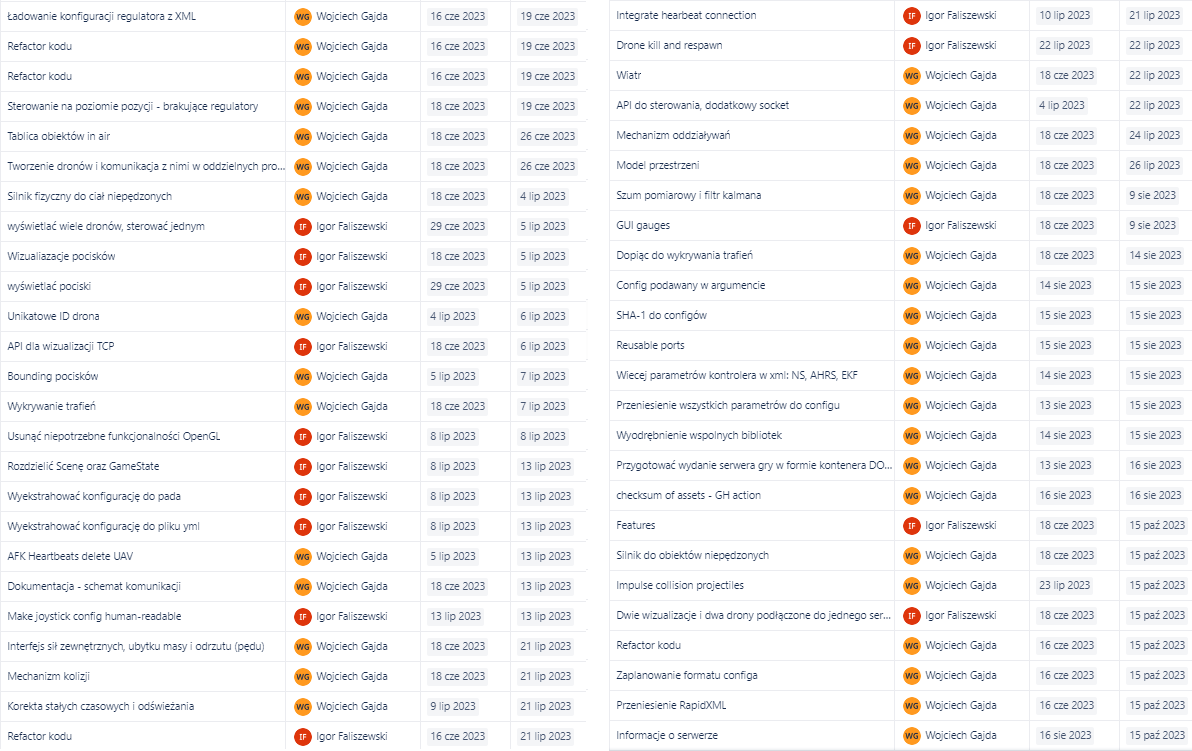
\includegraphics[width=\textwidth]{jira_june_sept.png}
\caption{Zgłoszenia zamknięte do 15.10.2023}
\label{zamkniete_jira}
\end{figure}

Na podstawie otwartych zagadnień i analizy założonej specyfikacji zaplanowany został harmonogram pracy zawierający zagadnienia których realizacja jest niezbędna do ukończenia projektu. Tabela (\ref{harmonogram}) prezentuje ww. harmonogram. 

\renewcommand{\arraystretch}{1.5}
\begin{table}
\centering
\begin{tabular}{|m{0.4\textwidth}|m{0.15\textwidth}|m{0.15\textwidth}|m{0.2\textwidth}|} 
\hline
\rowcolor{Gray}
Opis zadania & Data\newline rozpoczęcia & Data\newline zakończenia & Osoba\newline odpowiedzialna \\
 \hline
Dodanie różnych modeli pocisków i ładunków & 16.10.2023 & 23.10.2023 & Igor Faliszewski \\
 \hline
Dodanie nowych konfiguracji rakiet & 16.10.2023 & 29.10.2023 & Wojciech Gajda \\
 \hline
Generator konfiguracji kontrolera & 24.10.2023 & 29.10.2023 & Igor Faliszewski \\ 
\hline
Implementacja nowych regulatorów płatowców & 30.10.2023 & 19.11.2023 & Wojciech Gajda \\ 
\hline
Krzywa łańcuchowa & 30.10.2023 & 12.11.2023 & Igor Faliszewski \\ 
\hline
Określanie orientacji pocisków i~ładunków & 13.11.2023 & 19.11.2023 & Igor Faliszewski \\ 
\hline
GUI wyboru pocisku i ładunku & 20.11.2023 & 26.11.2023 & Igor Faliszewski \\ 
\hline
Rozwój klasy regulatorów PID & 20.11.2023 & 10.12.2023 & Wojciech Gajda \\ 
\hline
Radio & 27.11.2023 & 03.12.2023 & Igor Faliszewski \\ 
\hline
Generowanie assetów na podst. map terenu & 04.12.2023 & 31.12.2023 & Igor Faliszewski \\ 
\hline
Nazwy użytkowników nad statkami & 04.12.2023 & 10.12.2023 & Igor Faliszewski \\
 \hline
Dodatkowe algorytmy całkowania & 11.12.2023 & 31.12.2023 & Wojciech Gajda \\
 \hline
Dźwiek gry & 11.12.2023 & 18.12.2023 & Igor Faliszewski \\
 \hline
Limit FPS & 19.12.2023 & 23.12.2023 & Igor Faliszewski \\
 \hline
Zachowanie kamery w pobliżu ściany & 26.12.2023 & 31.12.2023 & Igor Faliszewski \\ 
\hline
Dokumentacja kodu & 16.10.2023 & 31.12.2023 & Wszyscy \\ 
\hline
Testy & 13.11.2023 & 31.12.2023 & Wszyscy \\
 \hline
Rozbudowa assetów & 30.10.2023 & 31.12.2023 & Wszyscy \\ 
\hline
\end{tabular}
\caption{Harmonogram projektu październik -- grudzień 2023}
\label{harmonogram}
\end{table}

\newpage
\subsection{Ocena ryzyka -- analiza SWOT}

\begin{table}[!h]
\begin{tikzpicture}
\renewcommand{\arraystretch}{1.2}
\setlist{left=1em,parsep=0.5ex,after=\smallskip}
\def\myw{7.5cm}
\matrix[SWOT] 
{
\& |[fill=black!10]|\renewcommand{\arraystretch}{1.3}\begin{tabular}{Wc{\myw}Wc{\myw}}
Pozytywne & Negatywne\\ 
\end{tabular}\\
 Wewnętrzne
  \& \begin{tabular}{p{\myw}p{\myw}}
	\textbf{Silne strony:} \begin{itemize}
 	 \item przejrzysta implementacja zgodna z paradygmatami programowania obiektowego,
        	 \item modułowość projektu, pozwalająca na modyfikację poszczególnych komponentów bez konieczności przebudowy całego projektu,
        	 \item uniwersalny model dynamiki statków powietrznych, pozwalający na obliczenia w czasie rzeczywistym.
\end{itemize}
& 
 \textbf{Słabe strony:} \begin{itemize}
  	\item ograniczony czas projektu może skutkować niedopracowaniami we wdrożonych funkcjonalnościach,
        \item obliczenia symulacji i kolizji obywają się na CPU, co może ograniczać wydajność,
        \item model matematyczny jest mniej dokładny niż rozbudowana symulacja mechaniki płynów.
\end{itemize} \end{tabular}\\
 Zewnętrzne \& \begin{tabular}{p{\myw}p{\myw}}
	\textbf{Szanse:} \begin{itemize}
   	\item dzięki udostępnieniu systemu na otwartej licencji, możliwe jest wykorzystanie wypracowanych rozwiązań w przyszłych projektach,
       	\item system może stanowić narzędzie ułatwiające opracowanie i testowanie nowatorskich systemów sterowania,
       	\item system może stanowić bezpłatną alternatywę dla komercyjnych symulatorów lotu.
\end{itemize} & \textbf{Zagrożenia:} \begin{itemize}
  \item język Rust wykorzystany w UAV\_aggregator może przestać być wspierany na przestrzeni najbliższych lat,
  \item trudności z identyfikacja wiarygodnych współczynników modelu dynamiki,
  \item rozbudowany system może okazać się trudny w obsłudze dla użytkownika.
  
\end{itemize} \end{tabular}\\
};
\end{tikzpicture}
\caption{Analiza SWOT}
\label{swot}
\end{table}

\newpage
\section{Testy oprogramowania}

Testowanie oprogramowania ma na celu weryfikację opracowanych rozwiązań. Odpowiednio przygotowane testy pozwalają na szybką detekcje błędu, a także rozwiązanie jego przyczyny. W zależności od przyjętej ideologi, testy oprogramowania przygotowywane są przed lub po opracowaniu własciwego kodu programu. Szczególnym przypadkiem testów pisanych po zakończeniu implementacji są testy pisane nigdy.\\

Metodyka realizacji testów dobrze rozwinięta dla typowych aplikacji webowych, co skutkuje dużym wyborem narzędzi umożliwijących testowanie i "mockowanie" modułów. W przypadku symulacji i gier komputerowych sytuacja jest odmienna. Oprócz sprawdzenia poprawności kodu niezbędna jest walidacja samego symulowanego modelu. Służą do tego specjalne mechanizmy, które wykształciły się w branży lotniczej.

Przygotowane testy można podzielić na trzy kategorie: testy jednostkowe, testy integracyjne oraz testy walidujące poprawność symulacji.

\subsection{Testy jednostkowe}

\subsection{Testy integracyjny}

\subsection{Testy walidujące}

\newpage
\section{Załączniki}

\begin{itemize} %[noitemsep,nolistsep]
\item UAV\_physic\_engine\_doc.pdf -- dokumentacja modułu UAV physic engine
\item UAV\_drop\_physic\_doc.pdf -- dokumentacja modułu UAV drop physic
\item UAV\_controller\_doc.pdf -- dokumentacja modułu UAV controller
\item UAV\_common\_doc.pdf -- dokumentacja wspólnej biblioteki dla modułów napisanych w języku C++
\item UAV\_aggregator\_doc.zip -- dokumentacja modułu UAV aggregator w formie strony HTML.
\item UAV\_visualization\_doc.zip -- dokumentacja modułu UAV visualization w formie strony HTML.

\item aircraft\_template.xml -- szablon pliku konfiguracyjnego statek powietrzny
\item aggregator\_config.yaml -- szablon pliku konfiguracyjnego modułu aggregator
\item visualization\_config.yaml -- szablon pliku konfiguracyjnego modułu wizualizacji
\item bindings\_template.yaml -- szablon pliku konfiguracyjnego kontroler
\item available\_control\_modes.yaml -- szablon pliku konfiguracyjnego trybów lotu
\end{itemize}


\newpage
\section{Bibliografia}

%\printbibliography
\nocite{*}

\printbibliography[type=book,heading=subbibliography,title={Literatura}]
\printbibliography[type=article,heading=subbibliography,title={Artykuły}]
\printbibliography[type=online,heading=subbibliography,title={Źródła internetowe}]

\end{document}\grid


\begin{comment}

Symulacje komputerowe dynamiki ruchu  W szczególności w zagadnieniu jakim jest projektowanie systemów sterowania do bezzałogowych statków powietrznych, zastosowanie takich narzędzi pozwala zminimalizować koszty wytworzenia poprawnie działającego systemu i przyśpieszyć jego rozwój i testowanie.

Celem niniejszej pracy jest opracowanie wirtualnego środowiska do symulacji dynamiki lotu bezzałogowych statków powietrznych. System implementuje podstawowy model dynamiki statków powietrznych wyposażonych w silniki rotorowe, silniki odrzutowe, powierzchnie nośne i powierzchnie sterowe. Pozwala na przeprowadzenie lotu symulowanym obiektem ktorego parametery określane są przez konfiguracje. System dzieli sie na serwer i aplikacje kliencką. Róznorodność modułów pozwala na realizacje róznych scenariusz (strzał, upuszczenie ładunku, kolizje, wpływ warunków srodowiskowych etc.)


\section{Model dynamiki statku powietrznego}

\begin{equation}
\begin{cases}
\dot{Y} =  T(Y) \cdot X + stabilizacja\\ 
A \cdot \dot{X} + \Omega (X) \cdot A \cdot X = F_g + F_a + F_d + F_o
\end{cases}
\end{equation}

gdzie:
\begin{itemize}
\item $Y$ - wektor pozycji i orientacji wyrażony w układzie globalnym
\item $X$ - wektor prędkości postępowej i kątowej w układzie związanym ze statkiem powietrznym
\item $A$ - macierz masowa
\item $\Omega$ - macierz gyroskopowa
\item $F_g$ - siła i moment pochodząca od siły grawitacji wyrażone w układzie związanym ze statkiem powietrznym
\item $F_a$ - siła i moment aerodynamiczny wyrażone w układzie związanym ze statkiem powietrznym
\item $F_d$ - siła i moment zespołów napędowych wyrażone w układzie związanym ze statkiem powietrznym
\item $F_o$ - siła i moment oddziaływań zewnętrznych napędowych wyrażone w układzie związanym ze statkiem powietrznym
\end{itemize}

\begin{equation}
Y = \begin{bmatrix}
x_{NED}\\
y_{NED}\\
z_{NED}\\
q_0\\
q_x\\
q_y\\
q_z
\end{bmatrix}
\end{equation}

\begin{equation}
X = \begin{bmatrix}
\dot{x}_b\\
\dot{y}_b\\
\dot{z}_b\\
P_b\\
Q_b\\
R_b
\end{bmatrix}
\end{equation}

\begin{equation}
F_g = R_{nb}(Y) \cdot  \begin{bmatrix}
0\\
0\\
g
\end{bmatrix}
\end{equation}

\begin{equation}
F_a = \frac{1}{2}\rho \cdot V_{tot}^2 S R_{wb} C_F \\
M_a = \frac{1}{2}\rho \cdot V_{tot}^2 S d R_{wb} C_F
\end{equation}

\end{comment}
